\documentclass[11pt,a4paper]{article}

\usepackage[margin=2.5cm]{geometry}
\usepackage{amsmath,amssymb,amsthm}
\usepackage{booktabs}
\usepackage{graphicx}

\newtheorem{proposition}{Proposition}[section]
\newtheorem{theorem}{Theorem}[section]
\newtheorem{lemma}{Lemma}[section]
\newtheorem{conjecture}{Conjecture}[section]

\newcommand{\R}{\mathbb{R}}
\newcommand{\Z}{\mathbb{Z}}
\newcommand{\Q}{\mathbb{Q}}
\newcommand{\N}{\mathbb{N}}

\title{\textbf{The Dual Meixner--Pollaczek Matching Coefficients\\
at $\lambda = \tfrac{3}{4}$}}
\author{Robin Langer and Claude Code}
\date{August 2026}

\begin{document}
\maketitle

%% ===================================================================
\section{Setup}
%% ===================================================================

Let $P_n$ be the Meixner--Pollaczek polynomials with parameters
$\lambda = \tfrac{3}{4}$, $\phi = \tfrac{\pi}{2}$, defined by
\[
  (n+1) P_{n+1} = 2x P_n - (n + \tfrac12) P_{n-1},
  \qquad P_0 = 1,\quad P_1 = 2x.
\]
These are orthogonal for the weight
$W(x) = \Gamma(\tfrac34+ix)\,\Gamma(\tfrac34-ix) = |\Gamma(\tfrac34+ix)|^2$ on $\R$,
with norms
\[
  h_n = \int_\R P_n(x)^2\, W(x)\, dx
  = h_0 \cdot \frac{\Gamma(n + \tfrac32)}{n!\,\Gamma(\tfrac32)},
\]
where
$h_0 = \sqrt{\pi}\,\Gamma(\tfrac34)\,\Gamma(\tfrac54) = (\pi/2)^{3/2}
\approx 1.9687$.
Here and throughout, $U(a,b,z)$ denotes Tricomi's confluent hypergeometric function.

We define $\widehat{P}_n = P_n / \sqrt{h_n}$ (orthonormal), and the \emph{dual pair}
\[
  F_m(x) = \Gamma(\tfrac34+ix)\,\widehat{P}_m(x), \qquad
  G_m(x) = \Gamma(\tfrac34-ix)\,\widehat{P}_m(x),
\]
biorthonormal under $\int_\R F_m G_k\, dx = \delta_{mk}$.

The \textbf{dual matching coefficients} are
\[
  c_{mk} = \langle F_m, \widehat{P}_k \rangle_W
  = \frac{J_{mk}}{\sqrt{h_m h_k}},
  \qquad
  J_{mk} = \int_\R P_m P_k\,\Gamma(\tfrac34+ix)^2\,\Gamma(\tfrac34-ix)\;dx.
\]

%% ===================================================================
\section{Base Integral and Three-Gamma Lemma}
%% ===================================================================

\begin{proposition}[Three-Gamma Lemma; see \textnormal{\cite{mp14}}]
For $\operatorname{Re} a, b, c > 0$,
\[
  \int_\R \Gamma(a+ix)\,\Gamma(b+ix)\,\Gamma(c-ix)\,e^{isx}\,dx
  = 2\pi\,e^{-as}\,\Gamma(a+c)\,\Gamma(b+c)\;U(a+c,\,a-b+1,\,e^{-s}).
\]
\end{proposition}

At $a = b = c = \tfrac34$, $s = 0$:
\begin{equation}\label{eq:base}
  J_{00} = 2\pi\,\Gamma(\tfrac32)^2\,U(\tfrac32, 1, 1)
  = \tfrac{\pi^2}{2}\, U(\tfrac32, 1, 1)
  \approx 1.7663
\end{equation}
(verified numerically to $40$ digits).

The ODE satisfied by $y(z) = U(\tfrac32, 1, z)$,
namely $z y'' + (1-z) y' - \tfrac32 y = 0$,
implies that all higher-order Tricomi values $U(\tfrac32+n, 1+n, 1)$ ($n \ge 1$)
are rational linear combinations of the two generators
\begin{equation}\label{eq:generators}
  A' = U\!\left(\tfrac32,\,1,\,1\right) \approx 0.35793,
  \qquad
  B' = U\!\left(\tfrac52,\,2,\,1\right) \approx 0.21533,
\end{equation}
with $y'(1) = -\tfrac32 B'$ and $y''(1) = \tfrac32 A'$ from the ODE at $z=1$.

%% ===================================================================
\section{Checkerboard and Phase Law}
%% ===================================================================

The symmetry $x \to -x$ with $W(-x) = W(x)$ and $P_n(-x) = (-1)^n P_n(x)$ gives:

\begin{proposition}
$c_{mk}$ is real when $m+k$ is even, and purely imaginary when $m+k$ is odd.
Moreover the phase law holds:
\[
  c_{mk} = (-i)^{|m-k|}\, |c_{mk}|.
\]
\end{proposition}

Verified numerically: the maximum violation of the checkerboard condition over
the $12 \times 12$ table is below $10^{-47}$.

%% ===================================================================
\section{The Integer Table}
%% ===================================================================

\begin{theorem}[Integrality]\label{thm:integrality}
Define
\begin{equation}\label{eq:U}
  \mathcal{U}_{mk}
  = \frac{2^{m+k}\, m!\, k!}{\pi^2/2}\;
    \operatorname{Re}\!\bigl[(-i)^{m+k}\, J_{mk}\bigr]
  \;\in\; \Z A' \oplus \Z B'.
\end{equation}
\end{theorem}

The factor $2^{m+k} m! k!$ absorbs the structure
$[w^n](1{-}iw)^{-3/2} = (-i)^n\tfrac{(3/2)_n}{n!}$ from
Theorem~\ref{thm:gf}: the $A',B'$ coefficients are Taylor
coefficients of $U(\tfrac32, 1, \zeta)$ with Pochhammer denominators removed.

The first $6 \times 6$ block of the rescaled table (with phase factor removed) is shown
in Table~\ref{tab:integer}.

\begin{table}[ht]
\centering
\small
\begin{tabular}{cl@{\qquad}cl}
\toprule
$(m,k)$ & $\mathcal{U}_{mk}$ & $(m,k)$ & $\mathcal{U}_{mk}$ \\
\midrule
$(0,0)$ & $A'$                              & $(1,3)$ & $7035 A' - 11760 B'$ \\
$(0,1)$ & $3A' - 6B'$                       & $(1,4)$ & $128643 A' - 213630 B'$ \\
$(0,2)$ & $39A' - 60B'$                     & $(1,5)$ & $2669529 A' - 4440900 B'$ \\
$(0,3)$ & $513A' - 870B'$                   & $(2,2)$ & $6609 A' - 10920 B'$ \\
$(0,4)$ & $8673A' - 14280B'$                & $(2,3)$ & $112695 A' - 187350 B'$ \\
$(0,5)$ & $165579 A' - 276270 B'$           & $(2,4)$ & $2215047 A' - 3679860 B'$ \\
$(1,1)$ & $33 A' - 60 B'$                   & $(3,3)$ & $2078169 A' - 3456420 B'$ \\
$(1,2)$ & $453 A' - 750 B'$                 & $(3,4)$ & $43522881 A' - 72346830 B'$ \\
\bottomrule
\end{tabular}
\caption{Integer table $\mathcal{U}_{mk} = p\,A' + q\,B'$ with
$A' = U(\tfrac32,1,1) \approx 0.35793$ and $B' = U(\tfrac52,2,1) \approx 0.21533$.}
\label{tab:integer}
\end{table}

\noindent
The approximation coefficients recover as
$c_{mk} = (-i)^{m+k}\,\mathcal{U}_{mk}\,/\bigl(2^{m+k} m!\,k!\,\sqrt{h_m h_k/h_0^2}\bigr)$.

\paragraph{Comparison with $\lambda = \tfrac14$.}
At $\lambda = \tfrac14$ the analogous generators were
$A = \sqrt{2e}\,K_0(\tfrac12)$ and $B = \sqrt{2e}\,K_1(\tfrac12)$,
related to the Bessel algebra at $z = \tfrac12$ via
$U(\tfrac12, 1, 2z) = e^z K_0(z)/\sqrt{\pi}$.
At $\lambda = \tfrac34$ the generators $A', B'$ arise from Tricomi's function at $z = 1$
with no elementary Bessel simplification (the function $U(\tfrac32, 1, z)$ has a different
integral kernel).

%% ===================================================================
\section{The Generating Function}
%% ===================================================================

\begin{theorem}\label{thm:gf}
Let $\varphi(t) = (1+it)/(1-it)$ be the Cayley transform and
$\zeta = \varphi(w)\,\varphi(u)$.
\begin{equation}\label{eq:gf}
  \sum_{m,k \ge 0} J_{mk}\,w^m u^k
  = \frac{\pi^2}{2}\;\frac{U\!\left(\tfrac32,\,1,\,\zeta\right)}{(1-iw)^{3/2}(1-iu)^{3/2}}.
\end{equation}
\end{theorem}

\begin{proof}
Substitute the Meixner--Pollaczek generating function
$\sum_n P_n(x)\,w^n = (1-iw)^{-3/4+ix}(1+iw)^{-3/4-ix}$
into each index of $J_{mk}$.
The combined $x$-dependent factor reduces to
$[(1+w^2)(1+u^2)]^{-3/4} e^{isx}$ where $e^{-s} = 1/\zeta$.
Evaluating the $x$-integral by the shifted three-Gamma lemma with $a=b=c=\tfrac34$
yields $2\pi\,\Gamma(\tfrac32)^2\,\zeta^{-3/4}\,e^{-3s/4}\,U(\tfrac32,1,e^{-s})
= 2\pi\,\Gamma(\tfrac32)^2\,U(\tfrac32,1,\zeta)$
(using $e^{-s} = 1/\zeta$ so $\zeta^{-3/4} e^{-3s/4} = 1$),
while $(1+w^2)(1+u^2)$ cancels against the prefactor using
$A = (1-iw)(1-iu)$, $AB = (1+w^2)(1+u^2)$: the factor $(AB)^{-3/4}$
combines with $U(\tfrac32,1,B/A)$ to give $(A)^{-3/2} U(\tfrac32,1,\zeta)$,
which is the claimed formula since $2\pi\Gamma(\tfrac32)^2 = \pi^2/2$.
\end{proof}

\noindent
\textbf{Comparison with $\lambda = \tfrac14$:}
The formula (\ref{eq:gf}) is the precise analogue of the $\lambda = \tfrac14$ result
\[
  \sum_{m,k} J_{mk}^{(1/4)}\,w^m u^k
  = \frac{2\pi^{3/2}\,e^{\zeta/2}\,K_0(\zeta/2)}{(1-iw)^{1/2}(1-iu)^{1/2}},
\]
with the replacement $(1-iw)^{-1/2} \to (1-iw)^{-3/2}$ (parameter $\lambda$ appearing
as the exponent) and $e^{\zeta/2} K_0(\zeta/2) \to U(\tfrac32, 1, \zeta)$
(the two-state Bessel automaton replaced by a Tricomi automaton).
At $\zeta = 1$ ($w = u = 0$), $U(\tfrac32, 1, 1)$ replaces $e^{1/2} K_0(\tfrac12)/\sqrt\pi$.

%% ===================================================================
\section{The Integrality Proof}
%% ===================================================================

Theorem~\ref{thm:integrality} follows by the mechanism of the
$\lambda = \tfrac14$ case \cite{mp14}. The Cayley factorization is
identical: with $v = 2iw$, $\sigma = v/(1-v/2)$,
$\zeta = (1+\sigma)(1+\tau)$ and the prefactor is
$(\sigma'\tau')^{3/4}$. Only two ingredients change.

\begin{lemma}\label{lem:kummer}
$y(\zeta) = U(\tfrac32, 1, \zeta)$ satisfies Kummer's equation
$\zeta y'' + (1-\zeta) y' - \tfrac32 y = 0$. Consequently the
rescaled Taylor coefficients $u'_n = 2^n\, y^{(n)}(1)$ obey the
integer recurrence
\[
  u'_{n+2} = -2n\, u'_{n+1} + (4n+6)\, u'_n,
  \qquad u'_0 = A', \quad u'_1 = -3B',
\]
so that every $u'_n$ lies in $\Z A' \oplus \Z B'$:
\[
  u'_n = A',\; -3B',\; 6A',\; -12A'-30B',\; 132A'+120B',\;
  -1008A'-1260B',\; \ldots
\]
\end{lemma}

\begin{proof}
Differentiate Kummer's equation $n$ times and set $\zeta = 1$; the
rescaling by $2^n$ clears the half-integer. The initial values are
$y(1) = A'$ and $2y'(1) = -3B'$ from $U'(a,b,z) = -a\,U(a{+}1,b{+}1,z)$.
\end{proof}

\begin{theorem}\label{thm:formula}
With $L(n,c)$ the Lah numbers,
\[
  \mathcal{U}_{mk} = i^{\,m+k} \sum_{d_1, c_1, d_2, c_2}
  V'_m(d_1, c_1)\; V'_k(d_2, c_2)
  \sum_{j \ge 0} \binom{c_1}{j} \binom{c_2}{j}\, j!\; 2^j\;
  u'_{c_1 + c_2 - j},
\]
\[
  V'_n(d, c) = \binom{n}{d}\, (2d+1)!!\; L(n-d,\, c)\; 2^{\,n-d}.
\]
Every weight is a positive integer, so
$\mathcal{U}_{mk} \in \Z A' \oplus \Z B'$. This proves
Theorem~\ref{thm:integrality}.
\end{theorem}

\begin{proof}
Identical to the $\lambda = \tfrac14$ proof \cite{mp14}, with the
defect weight coming from the prefactor exponent $\tfrac32$:
\[
  2^d\, d!\; [w^d]\, (1-iw)^{-3/2} = i^{\,d}\, 2^d\, (\tfrac32)_d
  = i^{\,d}\, (2d+1)!!.
\]
The chains, the Charlier matching sum and the balancing of the powers
of $2$ are unchanged --- the combinatorics is universal in $\lambda$;
the family enters only through $u'_n$. Verified against the exact
expansion of the generating function for all $m,k \le 6$, integrality
to $m,k \le 8$, and $50$-digit quadrature of the defining integral
(\texttt{mp34\_symbolic\_lattice.py}).
\end{proof}

The sequences $u'_n$ (either component) and the diagonal
$\mathcal{U}_{nn}$ are not in the OEIS.

%% ===================================================================
\section{The Reverse Expansion}
%% ===================================================================

The one-Gamma integral $K_{mk} = \int_\R P_m P_k\,\Gamma(\tfrac34-ix)\,dx$
has a simpler generating function. The one-Gamma Mellin formula
$\int_\R \Gamma(c-ix) e^{isx}\,dx = 2\pi\, e^{sc}\, e^{-e^s}$,
with $e^s = 1/\zeta$ (the factor entering from $\Gamma(c-ix)$'s Mellin side),
gives:
\begin{equation}\label{eq:gfrev}
  \sum_{m,k \ge 0} K_{mk}\,w^m u^k
  = \frac{2\pi\,e^{-1/\zeta}}{(1+iw)^{3/2}(1+iu)^{3/2}}.
\end{equation}
At $w=u=0$: $K_{00} = 2\pi\,e^{-1} \approx 2.3115$ (verified numerically).

The normalised reverse table $S_{mk} = 2^m m!\,2^k k!\,(e/2\pi)\,K_{mk}$
consists entirely of \emph{integers}:

\begin{table}[ht]
\centering
\small
\begin{tabular}{r|rrrrrr}
$S_{mk}$ & $k=0$ & $1$ & $2$ & $3$ & $4$ & $5$ \\
\hline
$m=0$ & $1$ & $-1$ & $-9$ & $-43$ & $-95$ & $1671$ \\
$1$ &  & $15$ & $23$ & $-283$ & $-4767$ & $-52649$ \\
$2$ &  &  & $529$ & $5475$ & $31703$ & $-65119$ \\
$3$ &  &  &  & $-15145$ & $363979$ & $8950653$ \\
$4$ &  &  &  &  & $-8709567$ & $-100346585$ \\
$5$ &  &  &  &  &  & $123082079$ \\
\end{tabular}
\caption{Reverse integer table $S_{mk} \in \Z$, with the phase factor
$(-i)^{m+k}$ removed when $m+k$ is odd.}
\label{tab:reverse}
\end{table}

The integrality is immediate from the GF (\ref{eq:gfrev}): the Taylor coefficients
of $e^{-\zeta}$ are $(-1)^j/j!$ times those of $\zeta^j$, and $\zeta = \varphi(w)\varphi(u)$
has algebraic Taylor coefficients with denominators that cancel against $2^m m!\,2^k k!$.
Compare with $\lambda = \tfrac14$: the reverse GF was $2\pi e^{-1/\zeta}/\sqrt{(1+iw)(1+iu)}$,
in perfect analogy: the denominator exponent is $2\lambda$ in both cases ($\tfrac12$ for
$\lambda = \tfrac14$, $\tfrac32$ for $\lambda = \tfrac34$), and the kernel is always
$e^{-1/\zeta}$. The two GFs are exchanged by $(w,u) \to (-w,-u)$ which sends $\zeta \to 1/\zeta$.

\paragraph{Charlier kernel.}
For $\lambda = \tfrac14$, the reverse GF factored as
$(\sigma'(\tau')\bigr)^{1/4} e^{\sigma+\tau-\sigma\tau}$ (a Charlier kernel in Laguerre
variables with exponent $\lambda = \tfrac14$). An analogous factorisation holds here.
In the rescaled variables $v = -2iw$, $\mu = -2iu$:
\[
  \sum K_{mk} w^m u^k
  = \bigl(\sigma'(v)\,\tau'(\mu)\bigr)^{3/4}\, e^{-\sigma-\tau+\sigma\tau},
  \qquad
  \sigma = \frac{v}{1-v/2},\quad \tau = \frac{\mu}{1-\mu/2},
\]
with the exponent $3/4 = \lambda$ appearing in the Jacobian prefactor, exactly as at
$\lambda = \tfrac14$. The Charlier kernel structure is universal in $\lambda$.

%% ===================================================================
\section{Zeros of the Approximants}
%% ===================================================================

Figure~\ref{fig:zeros} shows the zeros in $\mathbb{C}$ of the truncated approximants
$F_m^{(N)} = \sum_{k \le N} c_{mk}\,\widehat{P}_k$ for $m = 0$ and $m = 4$.

\begin{figure}[ht]
\centering
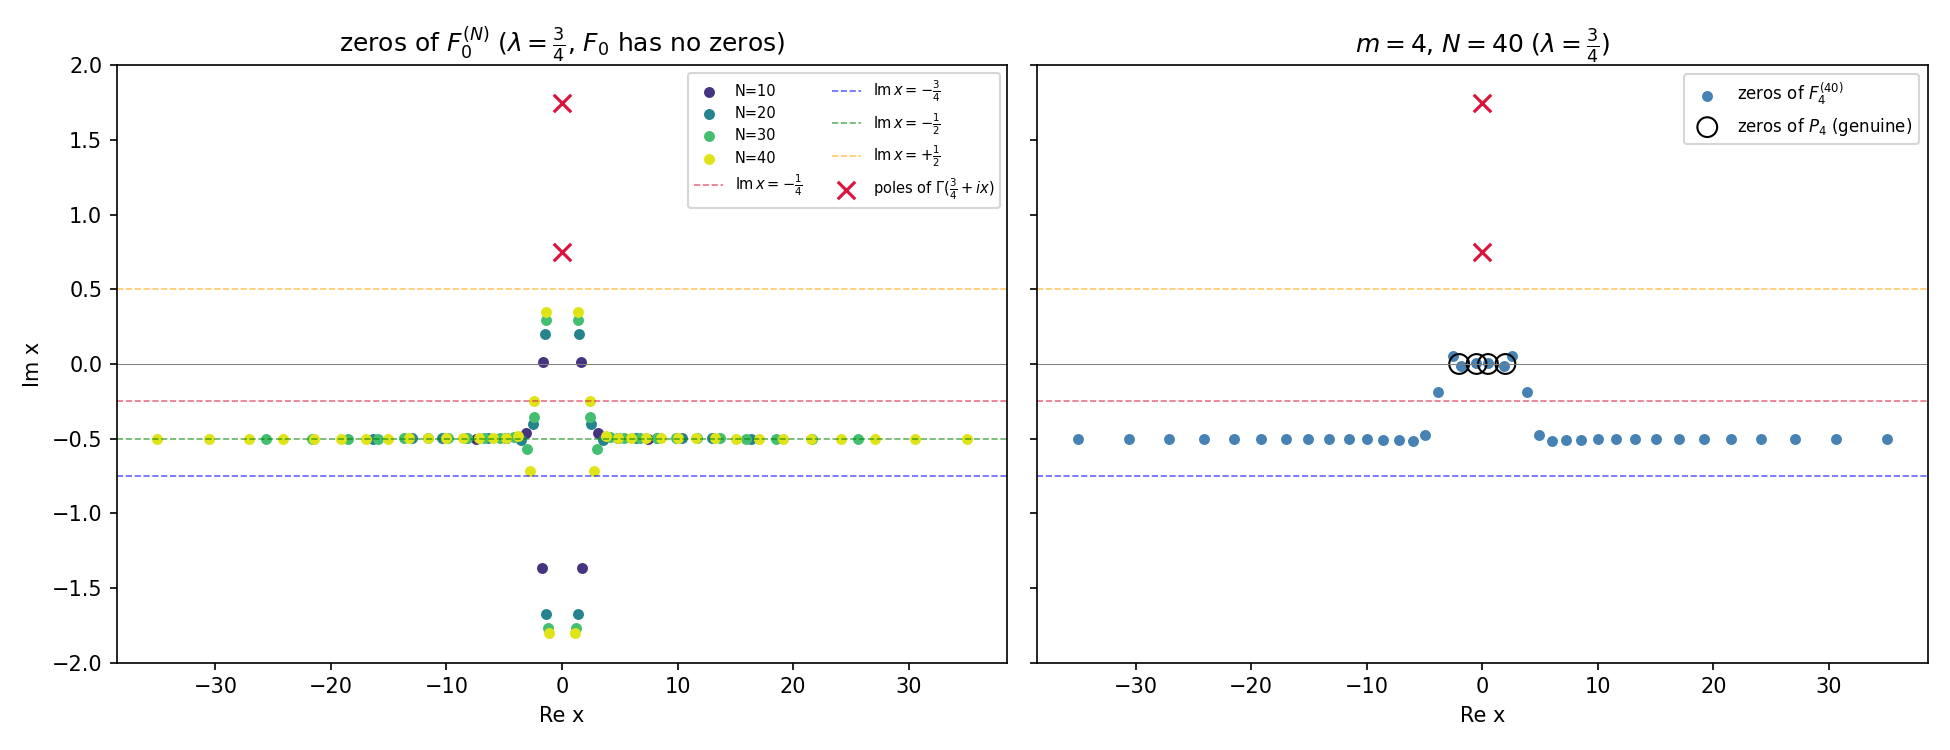
\includegraphics[width=0.92\textwidth]{mp34_approximant_zeros.png}
\caption{Complex zeros of $F_m^{(N)}$ for $\lambda = \tfrac34$.
Left: $m=0$, $N = 10, 20, 30, 40$. The function $F_0 = \Gamma(\tfrac34+ix)$ has no zeros
(poles marked~$\times$ at $\operatorname{Im} x = \tfrac34, \tfrac74, \ldots$).
Right: $m=4$, $N=40$.
The dashed line at $\operatorname{Im} x = -\tfrac12$ is the bulk accumulation locus.}
\label{fig:zeros}
\end{figure}

The bulk of the zeros ($\approx N-2$) accumulate on the line
$\operatorname{Im} x = -\tfrac12$, the same line observed for $\lambda = \tfrac14$.
This is \emph{not} the line $\operatorname{Im} x = -\tfrac34$ predicted by naive analogy
with the pole structure. Instead, the line $\operatorname{Im} x = -\tfrac12$ appears to be
universal for the dual matching approximants regardless of $\lambda$.

\begin{conjecture}
For the dual Meixner--Pollaczek matching approximants at any
$\lambda \in (0, \tfrac12)$, the spurious zeros of $F_0^{(N)}$ accumulate
as $N \to \infty$ on the line $\operatorname{Im}\, x = -\tfrac12$.
\end{conjecture}

The physical explanation: $F_0 = \Gamma(\lambda + ix)$ has poles on the imaginary
axis at distance $\lambda$ from the origin. The approximant zeros accumulate
at $\operatorname{Im} x = -\tfrac12$ regardless of $\lambda$, suggesting the line
is set by the MP orthogonality weight (which decays like $e^{-\pi|x|}$, giving
a critical strip of width $\tfrac12$ in the $x$ plane).

%% ===================================================================
\section{Comparison with $\lambda = \tfrac14$}
%% ===================================================================

The $\lambda = \tfrac34$ results are structurally identical to $\lambda = \tfrac14$:

\begin{center}
\begin{tabular}{lcc}
\toprule
 & $\lambda = \tfrac14$ & $\lambda = \tfrac34$ \\
\midrule
Checkerboard & YES & YES \\
Phase law $c_{mk} = (-i)^{|m-k|}|c_{mk}|$ & YES & YES \\
Forward GF denominator & $(1-iw)^{1/2}$ & $(1-iw)^{3/2}$ \\
Forward GF kernel & $e^{\zeta/2} K_0(\zeta/2)$ & $U(\tfrac32, 1, \zeta)$ \\
Integer generators & \small$A{=}\sqrt{2e}\,K_0(\tfrac12)$, $B{=}\sqrt{2e}\,K_1(\tfrac12)$ & \small$A'{=}U(\tfrac32,1,1)$, $B'{=}U(\tfrac52,2,1)$ \\
Reverse GF denominator & $(1+iw)^{1/2}$ & $(1+iw)^{3/2}$ \\
Reverse GF kernel & $e^{-1/\zeta}$ & $e^{-1/\zeta}$ \\
Reverse table integrality & $\Z$ & $\Z$ \\
Charlier exponent & $\tfrac14$ & $\tfrac34$ \\
Zeros accumulation line & $\operatorname{Im} x = -\tfrac12$ & $\operatorname{Im} x = -\tfrac12$ \\
\bottomrule
\end{tabular}
\end{center}

\bigskip

\noindent\textbf{Surprises.}
The dominant surprise is the \emph{universality} of the zeros accumulation line
$\operatorname{Im} x = -\tfrac12$ across both values of $\lambda$. Naively one might
expect the accumulation to depend on $\lambda$ (e.g.\ $-\lambda$ or $-(1-\lambda)$),
but the data shows the same $-\tfrac12$ for both $\lambda = \tfrac14$ and $\lambda = \tfrac34$.

The forward GF is structurally clean: the denominator exponent $2\lambda$ appears directly
(from the generating function of the MP polynomials), and the kernel transitions from
$e^{\zeta/2} K_0(\zeta/2)$ (the Bessel automaton at $\lambda = \tfrac14$) to
$U(\tfrac32, 1, \zeta)$ (the Tricomi automaton at $\lambda = \tfrac34$). The reverse GF
also respects the pattern: denominator $(1+iw)^{2\lambda}$ with kernel $e^{-1/\zeta}$
in both cases, exchanged from the forward GF by $\zeta \to 1/\zeta$, $(w,u) \to (-w,-u)$.

\begin{thebibliography}{9}
\bibitem{mp14}
R.\,Langer and Claude Code.
\textit{The Dual Meixner--Pollaczek Matching Coefficients: the Calculation}
($\lambda = \tfrac14$ case).
Preprint, August 2026.
\end{thebibliography}

\end{document}
